\documentclass{article}
\usepackage{import}
\usepackage{amsmath}
\usepackage{tabularray}
\usepackage{float}


\import{lib/latex/}{wgmlgz}
\patchcmd{\thebibliography}{\section*}{\section}{}{}

\begin{document}
\itmo[
      variant=13,
      labn=2,
      discipline=Вычислительная математика,
      group=P3212,
      student=Соколов Анатолий Владимирович,
      teacher=Наумова Надежда Александровна 
]
\lstset{language=rust}
\newgeometry{
  a4paper,
  top=20mm,
  right=10mm,
  bottom=20mm,
  left=30mm
}
\tableofcontents

\section{Обязательное задание}
\textbf{Программная реализация задачи:}
% \begin{enumerate}
	\begin{enumerate}
		\item Реализовать в программе методы по выбору пользователя
		\item \begin{itemize}
			\item Метод прямоугольников (3 модификации: левые, правые, средние)
			\item Метод трапеций
			\item Метод Симпсона
		\end{itemize}
		\item Методы должны быть оформлены в виде отдельной(ого) функции/класса.
		\item Вычисление значений функции оформить в виде отдельной(ого) функции/класса.
		\item Для оценки погрешности и завершения вычислительного процесса использо-
		вать правило Рунге.
		\item Предусмотреть вывод результатов: значение интеграла, число разбиения интервала интегрирования для достижения требуемой точности.
	\end{enumerate}
\textbf{Вычислительная реализация задачи}
\begin{enumerate}
	\item Вычислить интеграл, приведенный в таблице 1, точно.
	\item Вычислить интеграл по формуле Ньютона – Котеса при $n = 6$.
	\item Вычислить интеграл по формулам средних прямоугольников, трапеций и Симпсона при $n = 10$.
	\item Сравнить результаты с точным значением интеграла.
	\item Определить относительную погрешность вычислений для каждого метода.
	\item В отчете отразить последовательные вычисления.
\end{enumerate}
\section{Необязательное задание}
\begin{enumerate}
	\item Установить сходимость рассматриваемых несобственных интегралов 2 рода
	(2-3 функции). Если интеграл - расходящийся, выводить сообщение: «Интеграл
	не существует».
	
	\item Если интеграл сходящийся, реализовать в программе вычисление несобствен-
	ных интегралов 2 рода (заданными численными методами).
	
	\item Рассмотреть случаи, когда подынтегральная функция терпит бесконечный раз-
	рыв: 1) в точке a, 2) в точке b, 3) на отрезке интегрирования
\end{enumerate}

\subsection{Вариант}

Интеграл для вычислений в отчете: 
 $$\int_{1}^{3}(-2x^3-5x^2+7x-13)dx$$

\subsection{Цель работы}
      Найти приближенное значение определенного интеграла с требуемой точностью различными численными методами.

\section{Выполнение}

     \subsection{Точное вычисление интеграла:}
     
     $\displaystyle \int_{1}^{3}(-2x^3-5x^2+7x-13)dx 
      = \left(- \frac{x^4}{2} - \frac{5x^3}{3} + \frac{7x^2}{2}-13x\right)\biggr|_1^3
      = - \frac{244}{3} \approx -81.333$
      
    
     \subsection{Вычисление по формуле Ньютона – Котеса}
     
      Берём n=6, тогда коэффициенты Котеса для равноотстоящих узлов:
      \[c_6^0 = c_6^6 = \frac{42(b-a)}{840}\]
      \[c_6^1 = c_6^5 = \frac{216(b-a)}{840}\]
      \[c_6^2 = c_6^4 = \frac{27(b-a)}{840}\]
      \[c_6^3= \frac{272(b-a)}{840}\]
      \\
      Границы известны a=2; b=3:
      \[c_6^0 = c_6^6 = \frac{84}{840}\]
      \[c_6^1 = c_6^5 = \frac{432}{840}\]
      \[c_6^2 = c_6^4 = \frac{54}{840}\]
      \[c_6^3= \frac{544}{840}\]
      \\
      Найдём шаг разбиения:
      \[h = \frac{3-1}{6} = \frac{1}{3}\]
      \\
      Запишем определенный интеграл в виде:
      $$
      \int_{2}^{3}3x^3-2x^2-7x-8 = c_6^0\cdot f(a) 
      + c_6^1\cdot f(a+\frac{1}{3})
      + c_6^2\cdot f(a+\frac{2}{3}) 
      + c_6^3\cdot f(a+1)
      + c_6^4\cdot f(a+\frac{4}{3})
      + c_6^5\cdot f(a+\frac{5}{3})
      + c_6^6\cdot f(b)
      $$
      \[ f(1) = -13.0 \]
      \[ f(1 + \frac{1}{3}) = -17.296 \]
      \[ f(1 + \frac{2}{3}) = -24.481 \]
      \[ f(1 + 1) = -35.0 \]
      \[ f(1 + \frac{4}{3}) = -49.296 \]
      \[ f(1 + \frac{5}{3}) = -67.815 \]
      \[ f(3) = -91.0 \]
      $$
        \frac{84}{840} \cdot -13 
      + \frac{432}{840}\cdot -17.296
      + \frac{54}{840} \cdot -24.481
      + \frac{544}{840}\cdot -35.0
      + \frac{54}{840} \cdot -49.296
      + \frac{432}{840}\cdot -67.815
      + \frac{84}{840} \cdot -91.0
      \approx -81.58
      $$
      \\
      Относительная погрешность: 
      
      $$\varepsilon = \frac{|81.333-81.58|}{81.33}*100=0.3\%$$
      
      \subsection{Вычисление по формуле прямоугольников со средними высотами:}
      
      По условию дано n = 10, тогда делим отрезок интегрирования на 10 равных частей по формуле:
      \[h=\frac{b-a}{n} = \frac{3-1}{10} = 0.2\]
      \\
      По формуле средних прямоугольников:
      \[I = h\sum_{i=1}^{n}y_{i-\frac{1}{2}}\]
      \\
        
      \begin{table}[H]
      	\begin{center}
      		\begin{tabular}{|c|c|c|c|c|}
      			\hline
                $i$ & $x_i$ & $y_i$ & $x_{i-1/2}$ & $y_{i-1/2}$ \\ \hline
                 1 & 1.1 & -14.012 & 1.0 & -14.012 \\ \hline
                 2 & 1.3 & -16.744 & 1.2 & -16.744 \\ \hline
                 3 & 1.5 & -20.5 & 1.4 & -20.5 \\ \hline
                 4 & 1.7 & -25.376 & 1.6 & -25.376 \\ \hline
                 5 & 1.9 & -31.468 & 1.8 & -31.468 \\ \hline
                 6 & 2.1 & -38.872 & 2.0 & -38.872 \\ \hline
                 7 & 2.3 & -47.684 & 2.2 & -47.684 \\ \hline
                 8 & 2.5 & -58.0 & 2.4 & -58.0 \\ \hline
                 9 & 2.7 & -69.916 & 2.6 & -69.916 \\ \hline
                 10 & 2.9 & -83.528 & 2.8 & -83.528 \\ \hline
      		\end{tabular}
      		\caption{Приближенное вычисление интеграла методом средних прямоугольников}
      	\end{center}
      \end{table}
      
      \[I = 0.1\cdot (-14.012 -16.744 -20.5 -25.376 -31.468 -38.872 -47.684 -58.0 -69.916 -83.528) = -81.22\]
      \\
      Полученное для $n=10$ значение: $-81.22$.
      \\
      Относительная погрешность: 
      
      $$\varepsilon = \frac{|81.333-81.22|}{81.22}*100=0.139\%$$
      
      \subsection{Вычисление методом трапеций}
      
      По условия дано n = 10, тогда делим отрезок интегрирования на 10 равных частей по формуле:
      
      \[h=\frac{b-a}{n} = \frac{3-2}{10} = 0.1\]
      \\
      По формуле трапеций: 
      \[I = h\cdot \left(\frac{y_0+y_{10}}{2}+\sum_{i=1}^{n-1}y_i\right)\]

       \begin{table}[H]
      	\begin{center}
      		\begin{tabular}{|c|c|c|}
	      			\hline
	      			$i$ & $x_i$ & $y_i$ \\
	      			\hline
	      			0 & 1 & -13 \\
	      			1 & 1.2 & -15.256 \\
	      			2 & 1.4 & -18.488 \\
	      			3 & 1.6 & -22.792 \\
	      			4 & 1.8 & -28.264 \\
	      			5 & 2 & -35 \\
	      			6 & 2.2 & -43.096 \\
	      			7 & 2.4 & -52.648 \\
	      			8 & 2.6 & -63.752 \\
	      			9 & 2.8 & -76.504 \\
	      			10 & 3 & -91 \\
	      			\hline
      			\end{tabular}
      		\caption{Приближенное вычисление интеграла методом трапеций}
      	\end{center}
      \end{table}
      
      \[I = 0.1\cdot \left(\frac{-13-91}{2}+(-13 -15.256 -18.488 -22.792 -28.264 -35 -43.096 -52.648 -63.752 -76.504 -91)\right)\]
      \\
      Полученное для $n=10$ значение: $-81.56$.
      \\
      Относительная погрешность: 
      
      $$\varepsilon = \frac{|81.333-81.56|}{81.56}*100=0.279\%$$
      
      \subsection{Вычисление методом Симпсона}
      
       По условию дано n = 10, тогда делим отрезок интегрирования на 10 равных частей по формуле:
      \[h=\frac{b-a}{n} = \frac{3-1}{10} = 0.2\]
      \\
      По формуле Симпсона:
      \[I = \frac{h}{3}(y_0+ 4\cdot(y_1 + y_3+ y_5+ y_7+ y_9)+2\cdot(y_2 + y_4+ y_6+ y_8) + y_{10}) = \] 
      \begin{table}[H]
      	\begin{center}
      		\begin{tabular}{|c|c|c|}
	      		\hline
	      		$i$ & $x_i$ & $y_i$ \\
	      		\hline
	      		0 & 1 & -13 \\
	      		1 & 1.2 & -15.256 \\
	      		2 & 1.4 & -18.488 \\
	      		3 & 1.6 & -22.792 \\
	      		4 & 1.8 & -28.264 \\
	      		5 & 2 & -35 \\
	      		6 & 2.2 & -43.096 \\
	      		7 & 2.4 & -52.648 \\
	      		8 & 2.6 & -63.752 \\
	      		9 & 2.8 & -76.504 \\
	      		10 & 3 & -91 \\
	      		\hline
      		\end{tabular}
      		\caption{Приближенное вычисление интеграла методом Симпсона}
      	\end{center}
      \end{table}
      
      \[\frac{0.2}{3}(-13 + 4\cdot(-13 -18.488 -28.264 -43.096 -52.648 -76.504) + 2 \cdot (-18.488   -28.264   -43.096   -63.752 )  -91 = −68.252\]
      \\
      Относительная погрешность: 
      
      $$\varepsilon = \frac{|81.333-68.252|}{68.252}*100=16.247\%$$
      \subsection{Блок-схема реализованного алгоритма}
             \includegraphics[scale=0.15]{integration.png}
      \subsection{Ссылка на GitHub c основной реализацией}
            \href{https://github.com/isofinly/compmath}{Github}

      \subsection{Примеры и результаты работы программы}
            \begin{figure}[H] 
                  \begin{center}  
                         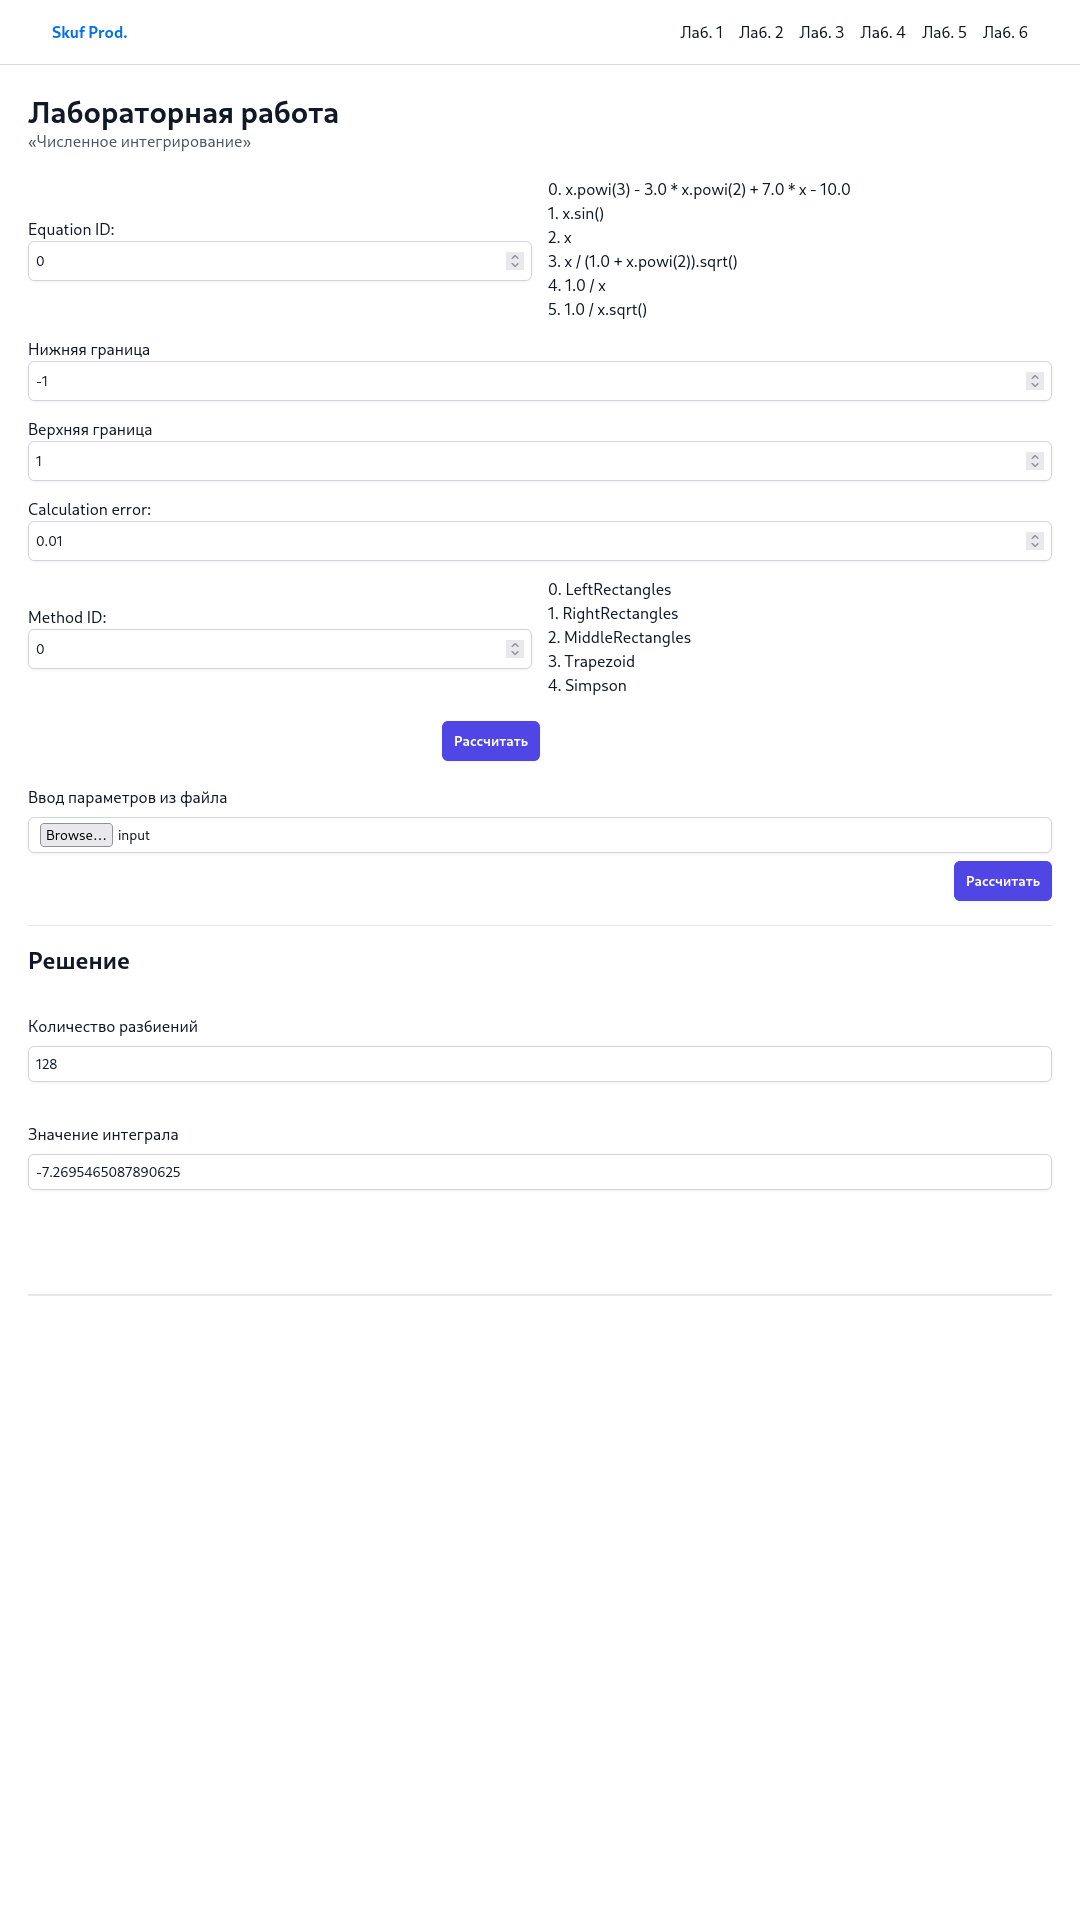
\includegraphics[scale=0.3]{ui2.png}
                        \caption{\small \sl {UI  1}}  
                  \end{center}  
            \end{figure}
            \begin{figure}[H] 
                  \begin{center}  
                         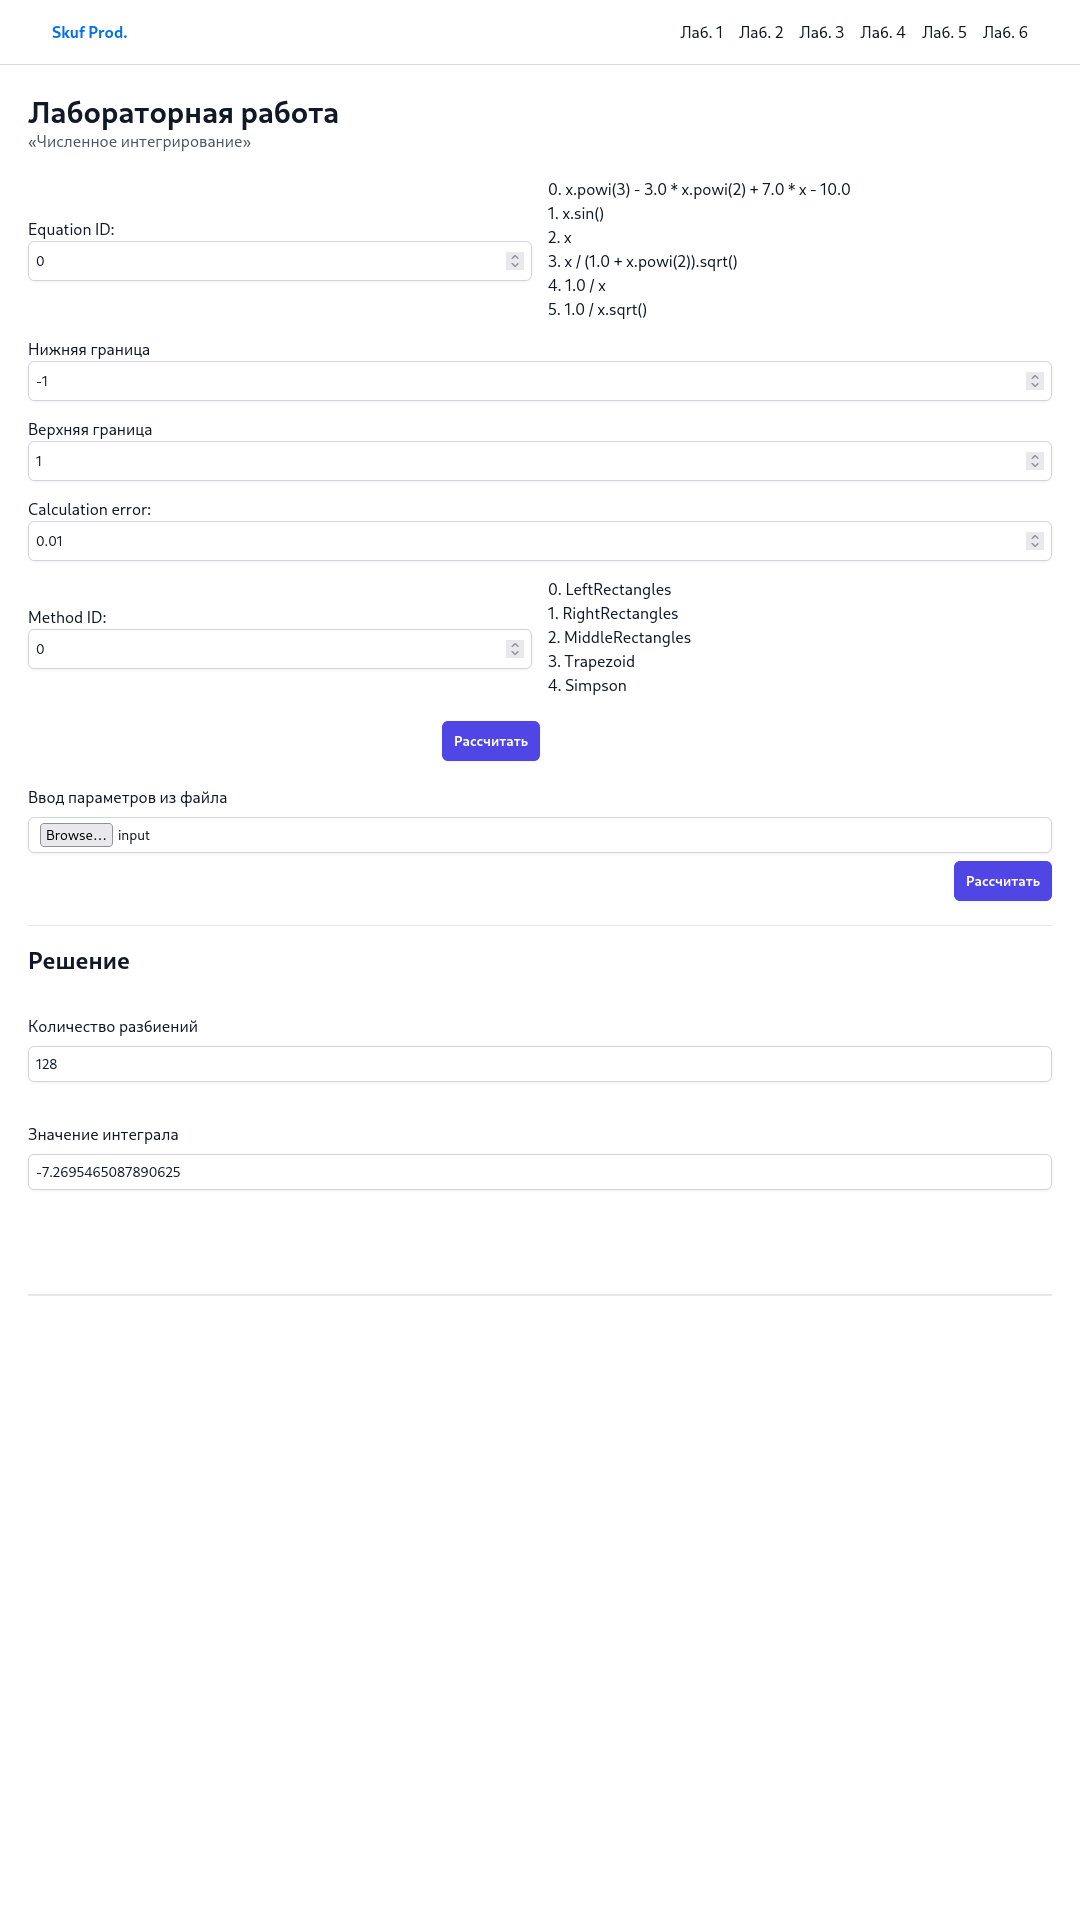
\includegraphics[scale=0.3]{ui2.png}
                        \caption{\small \sl {UI  2}}  
                  \end{center}  
            \end{figure}

\section{Заключение}
      В ходе выполнения данной ЛР я ознакомился с основыми методами интегрирования. Вообще с кайфом написал даже не 2к строк кода, а всего 800

\begin{thebibliography}{9}
    \bibitem{Методичка}Слайды с лекций (2023). // Кафедра информатики и вычислительной техники -- Малышева Татьяна Алексеевна, к.т.н., доцент.
\end{thebibliography} 

\end{document}
